\documentclass[tikz, border=12pt]{standalone}
\usepackage{amsmath}
\usetikzlibrary{positioning, arrows.meta}
\begin{document}
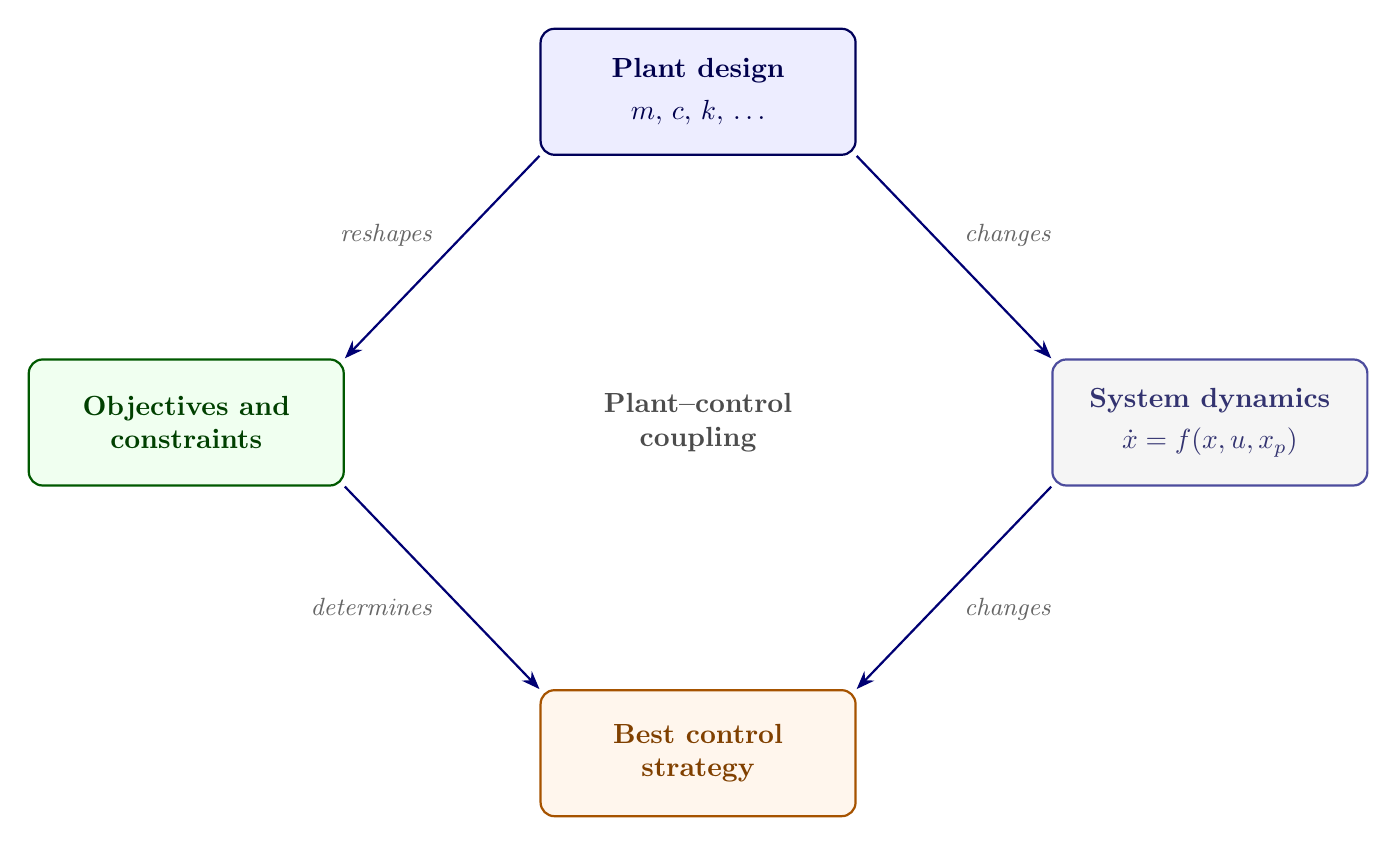
\begin{tikzpicture}[
    font=\sffamily,
    >=Stealth,
    vertex/.style={rectangle, rounded corners=5pt, thick, align=center,
        minimum width=4.0cm, minimum height=1.6cm, inner sep=6pt, font=\bfseries},
    sig/.style={font=\itshape\small, text=black!60},
]

% ---- Diamond vertex positions ----
% top = Plant design, right = System dynamics,
% bottom = Best control strategy, left = Objectives and constraints
\node[vertex, draw=blue!35!black, fill=blue!7, text=blue!30!black] (top)
    at (0,4.2) {Plant design\\[3pt] \normalfont\itshape $m,\,c,\,k,\,\ldots$};

\node[vertex, draw=blue!45!black!70, fill=black!4, text=blue!30!black!80] (right)
    at (6.5,0) {System dynamics\\[3pt] \normalfont\itshape $\dot{x} = f(x,u,x_p)$};

\node[vertex, draw=orange!65!black, fill=orange!7, text=orange!50!black] (bottom)
    at (0,-4.2) {Best control\\ strategy};

\node[vertex, draw=green!35!black, fill=green!6, text=green!25!black] (left)
    at (-6.5,0) {Objectives and\\ constraints};

% ---- Center label ----
\node[font=\bfseries, align=center, text=black!70] (center) at (0,0)
    {Plant--control\\ coupling};

% ---- Diamond edges (arrows) ----
\draw[->, thick, blue!45!black] (top.south west) -- (left.north east)
    node[midway, sig, above left] {reshapes};
\draw[->, thick, blue!45!black] (top.south east) -- (right.north west)
    node[midway, sig, above right] {changes};
\draw[->, thick, blue!45!black] (right.south west) -- (bottom.north east)
    node[midway, sig, below right] {changes};
\draw[->, thick, blue!45!black] (left.south east) -- (bottom.north west)
    node[midway, sig, below left] {determines};

\end{tikzpicture}
\end{document}
